\documentclass[a4paper,12pt,french]{article}

\usepackage[cours]{../../Style}

% Début du document
%%%%%%%%%%%%%%%%%%%
\begin{document}

\title{Fonctions: Généralités}
\maketitle

%\begin{FlushLeft}

\section{Définitions, notations, représentation}

\begin{defin}
Soit $D \subset \R$. On appelle fonction $f$ sur l'ensemble $D$ le processus qui à tout nombre $x \in D$ associe un unique réel noté $f(x)$. On note $\fonction f D {\R} x {f(x)}$. On dit alors que:
\begin{itemize}
\item $f(x)$ est l'image de $x$
\item $x$ est un antécédent de $f(x)$
\item $D$ est l'ensemble ( ou domaine ) de définition de $f$
\end{itemize}
\end{defin}

\begin{ex}
On définit la fonction $\fonction f {\R} {\R} x {x^2-x}$.
\begin{itemize}
\item L'image de $2$ par la fonction $f$ est $2$: $f(2)=2^2-2=2$.
\item $2$ est un antécédent de $2$ par la fonction $f$. $-1$ en est aussi un car $f(-1)=(-1)^2+1=2$.
\end{itemize}
\end{ex}

\begin{rmq}
Chaque nombre dans $D$ possède une unique image, mais plusieurs antécédents d'un même nombre peuvent exister.
\end{rmq}

\begin{defin}
Dans un repère du plan, l'ensemble des points $(x,f(x))$ pour $x \in D$ constitue la courbe de $f$. L'équation de la courbe de $f$ est $y=f(x)$ pour $x \in D$.
\end{defin}

\begin{methode}
Dans la pratique, il faut placer plusieurs points pour tracer la courbe d'une fonction le plus précisément possible. On peut s'aider d'une table de valeurs.
\end{methode}

\begin{ex}
\begin{center}
\begin{tabularx}{0.95\linewidth}{ 
  | >{\centering\arraybackslash}c 
  | >{\centering\arraybackslash}X
  | >{\centering\arraybackslash}X
  | >{\centering\arraybackslash}X
  | >{\centering\arraybackslash}X
  | >{\centering\arraybackslash}X
  | >{\centering\arraybackslash}X
  | >{\centering\arraybackslash}X
  | >{\centering\arraybackslash}X
  | >{\centering\arraybackslash}X| } \hline
$x$ & $-1.5$ & $-1$ & $-0.5$ & $0$ & $0.5$ & $1$ & $1.5$ & $2$ & $2.5$ \\ \hline
$f(x)$ & & & & & & & & &\rule[-7pt]{0pt}{30pt} \\ \hline
\end{tabularx}
\end{center}

\begin{center}
\begin{tikzpicture}
\begin{axis}[
styleglobal,
width=0.9*\linewidth,
xmin=-4, xmax=4,
ymin=-1, ymax=4,
xtick distance=1,
ytick distance=1,
]
\addplot[styleplot] {x^2-x} node [pos=0.85,right] {$\mathscr C_f$};
\addlegendentry{$f(x)=x^2-x$};
\pgfplotsinvokeforeach{-1.5,-1,...,2.5}{\node[stylepoint,fill=red] at (#1,#1*#1-#1) {};}
\draw[color=blue,dashed,very thick] (2.2, 0) -- (2.2, 2.2^2-2.2) node [pos=0,below] {$x$};
\draw[color=blue,dashed,very thick] (2.2, 2.2^2-2.2) -- (0, 2.2^2-2.2) node [pos=1,left] {$f(x)$};
\node[stylepoint] at (2.2,2.2^2-2.2) {};
%\addplot +[mark=none,color=red,style=dashed,very thick] coordinates {(-1, 0) (-1, 2)};
%\addplot +[mark=none,color=red,style=dashed,very thick] coordinates {(-1, 2) (0, 2)};
%\node[label={0:{$(0,1)$}},rectangle,fill,inner sep=2pt] at (axis cs:0,1) {};
%\node[label={[label distance=2pt]-90:{$(0,1)$}},rectangle,fill,inner sep=0pt, minimum height=0pt, minimum width=4pt] at (axis cs:1,1) {};
\end{axis}
\end{tikzpicture}
\end{center}
\end{ex}

\rem{Exos 101 -> 104 p32}
\section{Résolution graphique d'équations et d'inéquations}

\subsection{Equations}

\begin{methode}
\begin{center}
\begin{tabularx}{1\linewidth}{|X|X|} \hline
\Centering \begin{tikzpicture}[scale=1]
\begin{axis}[
axis x line=bottom,
axis y line = left,
axis lines=middle,
width=1.1*\linewidth,
height=0.75*\linewidth,
xmin=-0.5, xmax=4.5,
ymin=-0.5, ymax=4,
enlargelimits={abs=0.2},
xlabel={$x$},
ylabel={$y$},
%ytick distance=1,
ticks=none,
grid style=dashed,
%axis equal,
legend pos=north east,
xlabel style={at={(ticklabel* cs:0.95)},below=0.1},
]
\addplot[samples=101,smooth,ultra thick,domain=(-2:5),mark=none]{3.5*e^(-0.4*(x-2)^2)} node [pos=0.75,right] {$\mathscr C_f$};

\addplot +[mark=none,color=blue,style=dashed,very thick] coordinates {(-1,2.8) (5, 2.8)} node [pos=0.18,above right] {$k$};
\node[circle, minimum size=1pt,fill,color=blue,inner sep=2pt] at (axis cs:1.25,2.8) {};
\node[circle, minimum size=1pt,fill,color=blue,inner sep=2pt] at (axis cs:2.75,2.8) {};
\addplot +[mark=none,color=blue,style=dashed,very thick] coordinates {(1.25,0) (1.25, 2.8)} node [pos=0,below] {$a$};
\addplot +[mark=none,color=blue,style=dashed,very thick] coordinates {(2.75,0) (2.75, 2.8)} node [pos=0,below] {$b$};
%\addplot +[mark=none,color=red,style=dashed,very thick] coordinates {(-1, 0) (-1, 2)};
%\addplot +[mark=none,color=red,style=dashed,very thick] coordinates {(-1, 2) (0, 2)};
%\node[label={0:{$(0,1)$}},rectangle,fill,inner sep=2pt] at (axis cs:0,1) {};
%\node[label={[label distance=2pt]-90:{$(0,1)$}},rectangle,fill,inner sep=0pt, minimum height=0pt, minimum width=4pt] at (axis cs:1,1) {};
\end{axis}
\end{tikzpicture}
&
\Centering 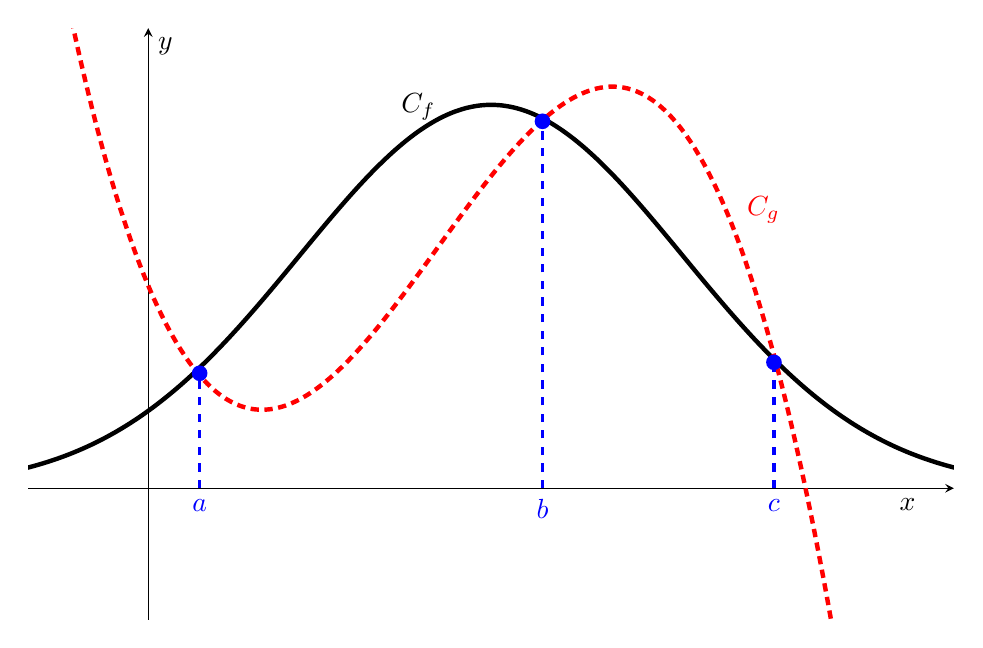
\begin{tikzpicture}[scale=1]
\begin{axis}[
axis x line=bottom,
axis y line = left,
axis lines=middle,
width=1.1*\linewidth,
height=0.75*\linewidth,
xmin=-0.5, xmax=4.5,
ymin=-1, ymax=4,
enlargelimits={abs=0.2},
xlabel={$x$},
ylabel={$y$},
ticks=none,
%ytick distance=1,
%axis equal,
yticklabel=\empty,
xticklabel=\empty,
xlabel style={at={(ticklabel* cs:0.95)},below=0.1},
]
\addplot[samples=101,smooth,ultra thick,domain=(-2:5),mark=none]{3.5*e^(-0.4*(x-2)^2)} node [pos=0.5,above] {$\mathscr C_f$};
\addplot[samples=101,smooth,ultra thick,domain=(-2:5),mark=none,color=red, densely dashed]{-0.69*x^3+3.49*x^2-3.72*x+1.85} node [pos=0.65,above right,color=red] {$\mathscr C_g$};

\addplot +[mark=none,color=blue,style=dashed,very thick] coordinates {(0.3,0) (0.3, 1.05)} node [pos=0,below] {$a$} node[pos=1,circle, minimum size=1pt,fill,inner sep=2pt] {};
\addplot +[mark=none,color=blue,style=dashed,very thick] coordinates {(2.3,0) (2.3, 3.35)} node [pos=0,below] {$b$} node[pos=1,circle, minimum size=1pt,fill,inner sep=2pt] {};
\addplot +[mark=none,color=blue,style=dashed,very thick] coordinates {(3.65,0) (3.65, 1.15)} node [pos=0,below] {$c$} node[pos=1,circle, minimum size=1pt,fill,inner sep=2pt] {};
%\addplot +[mark=none,color=red,style=dashed,very thick] coordinates {(-1, 0) (-1, 2)};
%\addplot +[mark=none,color=red,style=dashed,very thick] coordinates {(-1, 2) (0, 2)};
%\node[label={0:{$(0,1)$}},rectangle,fill,inner sep=2pt] at (axis cs:0,1) {};
%\node[label={[label distance=2pt]-90:{$(0,1)$}},rectangle,fill,inner sep=0pt, minimum height=0pt, minimum width=4pt] at (axis cs:1,1) {};
\end{axis}
\end{tikzpicture}
\\ \hline
Résoudre l'équation $f(x)=k$ signifie trouver les antécédents de $k$ par la fonction $f$.
Cela revient donc à chercher l'abscisse des points de la courbe dont l'ordonnée est $k$.

Ici, l'ensemble des solution de l'équation est:$$S=\{a;b \}$$
&
Résoudre l'équation $f(x)=g(x)$ signifie trouver les nombres qui ont la même image par $f$ et $g$.
Cela revient donc à chercher l'abscisse des points d'intersection des deux courbes $\mathscr C_f$ et $\mathscr C_g$.

Ici, l'ensemble des solution de l'équation est:$$S=\{ a;b;c \}$$ \\ \hline
\end{tabularx}
\end{center}
\end{methode}

\begin{exs}
\begin{center}
\begin{tabularx}{1\linewidth}{|Y|Y|Y|} \hline
\begin{tikzpicture}
\begin{axis}[
styleglobal,
width=0.9*\linewidth,
xmin=-5, xmax= 5,
ymin=-2, ymax=5,
xtick distance=1,
ytick distance=1,
minor x tick num=0,
minor y tick num=0,
%tick label style = {font=\scriptsize},
]
\addplot[styleplot] plot coordinates {(-4,2) (-2,-1) (0,0) (2,3) (4,0.5)};
\end{axis}
\end{tikzpicture}
&
\begin{tikzpicture}
\begin{axis}[
styleglobal,
width=0.9*\linewidth,
xmin=-2, xmax= 8,
ymin=-2, ymax=5,
xtick distance=1,
ytick distance=1,
minor x tick num=0,
minor y tick num=0,
%tick label style = {font=\scriptsize},
]
\addplot[styleplot] plot coordinates {(-1,4) (4,2) (5,4) (7,-1.5)};
\end{axis}
\end{tikzpicture}
&
\begin{tikzpicture}
\begin{axis}[
styleglobal,
width=0.9*\linewidth,
xmin=-7, xmax= 3,
ymin=-5, ymax=2,
xtick distance=1,
ytick distance=1,
minor x tick num=0,
minor y tick num=0,
%tick label style = {font=\scriptsize},
]
\addplot[styleplot] plot coordinates {(-6,1) (-3,-3) (-2,0) (2,-3.5)};
\end{axis}
\end{tikzpicture}
\\ \hline
Résoudre $f(x)=1$:
\rule[-1cm]{0pt}{1cm}
&
Résoudre $g(x)=1$:
\rule[-1cm]{0pt}{1cm}
&
Résoudre $h(x)=-4$:
\rule[-1cm]{0pt}{1cm} \\ \hline
\begin{tikzpicture}
\begin{axis}[
styleglobal,
width=0.9*\linewidth,
xmin=-5, xmax= 5,
ymin=-2, ymax=5,
xtick distance=1,
ytick distance=1,
minor x tick num=0,
minor y tick num=0,
%tick label style = {font=\scriptsize},
]
\addplot[styleplot] plot coordinates {(-4,2) (-2,-1) (0,0) (2,3) (4,0.5)} node[pos=0.8,above right] {$\mathscr C_{f_1}$};
\addplot[styleplot,color=blue,densely dashed] plot coordinates {(-4,4) (4,-1)} node[pos=0.75,above right] {$\mathscr C_{f_2}$};
\end{axis}
\end{tikzpicture}
&
\begin{tikzpicture}
\begin{axis}[
styleglobal,
width=0.9*\linewidth,
xmin=-2, xmax= 8,
ymin=-2, ymax=5,
xtick distance=1,
ytick distance=1,
minor x tick num=0,
minor y tick num=0,
%tick label style = {font=\scriptsize},
]
\addplot[styleplot] plot coordinates {(-1,4) (1,2) (4,1) (6,4) (7,2)} node[pos=0.9,above right] {$\mathscr C_{g_1}$};
\addplot[styleplot,color=blue,densely dashed] plot coordinates {(-1,1) (3,4) (7,1)} node[pos=0.5,above right] {$\mathscr C_{g_2}$};
\end{axis}
\end{tikzpicture}
&
\begin{tikzpicture}
\begin{axis}[
styleglobal,
width=0.9*\linewidth,
xmin=-7, xmax= 3,
ymin=-5, ymax=2,
xtick distance=1,
ytick distance=1,
minor x tick num=0,
minor y tick num=0,
%tick label style = {font=\scriptsize},
]
\addplot[styleplot] plot coordinates {(-6,1) (-3,-3) (-2,0) (2,-3.5)} node[pos=0.8,above right] {$\mathscr C_{h_1}$};
\addplot[styleplot,color=blue,densely dashed] plot coordinates {(-6,0) (-3,-4) (-1.5,-1) (2,-4.5)} node[pos=0.95,below left] {$\mathscr C_{h_2}$};
\end{axis}
\end{tikzpicture}
\\ \hline
Résoudre $f_1(x)=f_2(x)$:
\rule[-1cm]{0pt}{1cm}
&
Résoudre $g_1(x)=g_2(x)$:
\rule[-1cm]{0pt}{1cm}
&
Résoudre $h_1(x)=h_2(x)$:
\rule[-1cm]{0pt}{1cm} \\ \hline
\end{tabularx}
\end{center}
\end{exs}

\subsection{Inéquations}

\renewcommand\tabularxcolumn[1]{p{#1}}
\begin{methode}
\begin{center}
\begin{tabularx}{\linewidth}{|X|X|X|} \hline
\Centering{$f(x)>k$} & \Centering{$f(x) \leq k$} & \Centering{$f(x)>g(x)$} \\ \hline
\multicolumn{2}{|c|}{
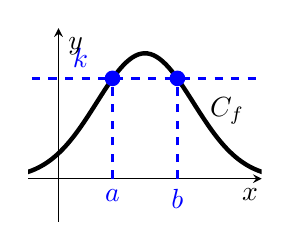
\begin{tikzpicture}[scale=1]
\begin{axis}[
axis x line=bottom,
axis y line = left,
axis lines=middle,
width=0.375*\linewidth,
height=0.333*\linewidth,
xmin=-0.5, xmax=4.5,
ymin=-1, ymax=4,
enlargelimits={abs=0.2},
xlabel={$x$},
ylabel={$y$},
%ytick distance=1,
ticks=none,
grid style=dashed,
%axis equal,
legend pos=north east,
xlabel style={at={(ticklabel* cs:0.95)},below=0.1},
]
\addplot[samples=101,smooth,ultra thick,domain=(-2:5),mark=none]{3.5*e^(-0.4*(x-2)^2)} node [pos=0.75,right] {$\mathscr C_f$};

\addplot +[mark=none,color=blue,style=dashed,very thick] coordinates {(-1,2.8) (5, 2.8)} node [pos=0.18,above right] {$k$};
\node[circle, minimum size=1pt,fill,color=blue,inner sep=2pt] at (axis cs:1.25,2.8) {};
\node[circle, minimum size=1pt,fill,color=blue,inner sep=2pt] at (axis cs:2.75,2.8) {};
\addplot +[mark=none,color=blue,style=dashed,very thick] coordinates {(1.25,0) (1.25, 2.8)} node [pos=0,below] {$a$};
\addplot +[mark=none,color=blue,style=dashed,very thick] coordinates {(2.75,0) (2.75, 2.8)} node [pos=0,below] {$b$};
%\addplot +[mark=none,color=red,style=dashed,very thick] coordinates {(-1, 0) (-1, 2)};
%\addplot +[mark=none,color=red,style=dashed,very thick] coordinates {(-1, 2) (0, 2)};
%\node[label={0:{$(0,1)$}},rectangle,fill,inner sep=2pt] at (axis cs:0,1) {};
%\node[label={[label distance=2pt]-90:{$(0,1)$}},rectangle,fill,inner sep=0pt, minimum height=0pt, minimum width=4pt] at (axis cs:1,1) {};
\end{axis}
\end{tikzpicture}}
&
\Centering{
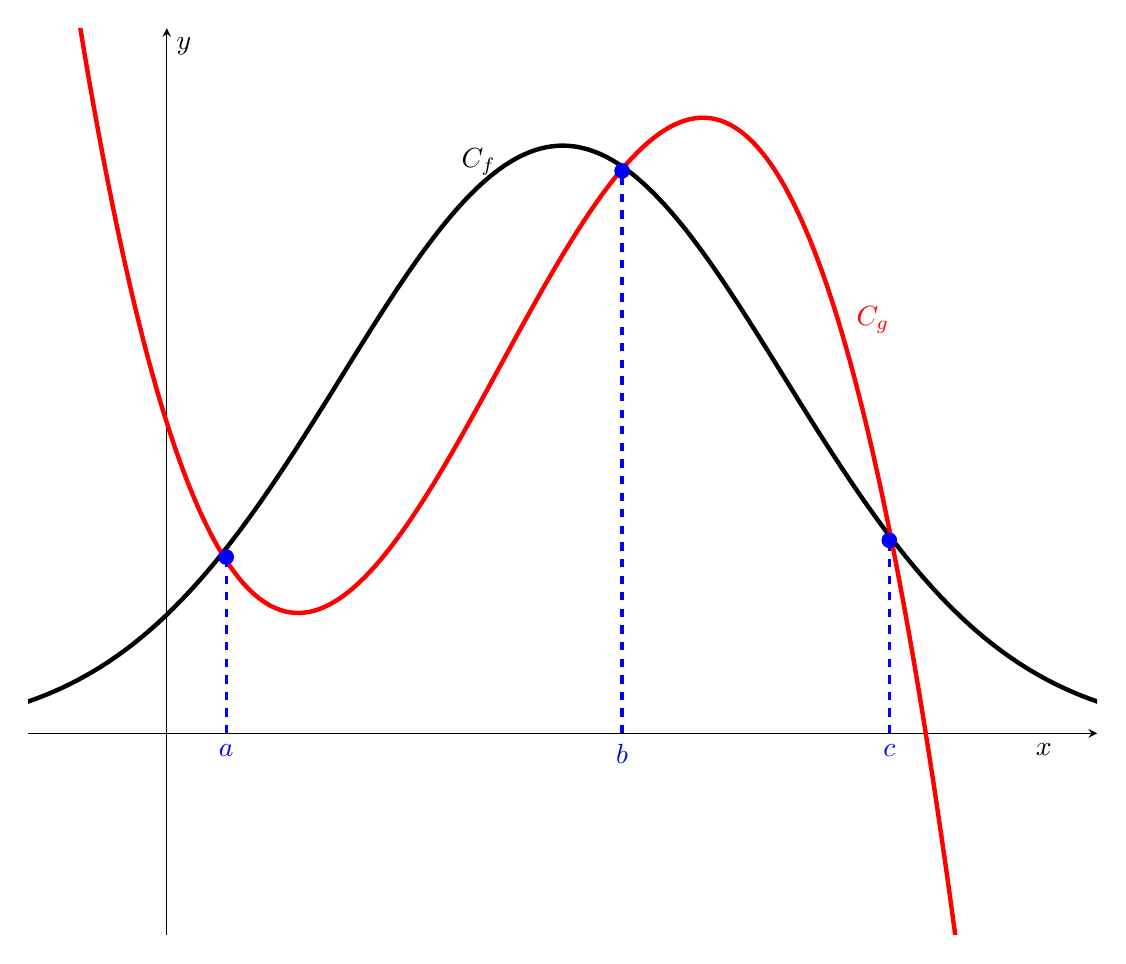
\begin{tikzpicture}[scale=1]
\begin{axis}[
axis x line=bottom,
axis y line = left,
axis lines=middle,
width=1.25*\linewidth,
height=1.08*\linewidth,
xmin=-0.5, xmax=4.5,
ymin=-1, ymax=4,
enlargelimits={abs=0.2},
xlabel={$x$},
ylabel={$y$},
ticks=none,
%ytick distance=1,
%axis equal,
yticklabel=\empty,
xticklabel=\empty,
xlabel style={at={(ticklabel* cs:0.95)},below=0.1},
]
\addplot[samples=101,smooth,ultra thick,domain=(-2:5),mark=none]{3.5*e^(-0.4*(x-2)^2)} node [pos=0.5,above] {$\mathscr C_f$};
\addplot[samples=101,smooth,ultra thick,domain=(-2:5),mark=none,color=red]{-0.69*x^3+3.49*x^2-3.72*x+1.85} node [pos=0.65,above right,color=red] {$\mathscr C_g$};

\addplot +[mark=none,color=blue,style=dashed,very thick] coordinates {(0.3,0) (0.3, 1.05)} node [pos=0,below] {$a$} node[pos=1,circle, minimum size=1pt,fill,inner sep=2pt] {};
\addplot +[mark=none,color=blue,style=dashed,very thick] coordinates {(2.3,0) (2.3, 3.35)} node [pos=0,below] {$b$} node[pos=1,circle, minimum size=1pt,fill,inner sep=2pt] {};
\addplot +[mark=none,color=blue,style=dashed,very thick] coordinates {(3.65,0) (3.65, 1.15)} node [pos=0,below] {$c$} node[pos=1,circle, minimum size=1pt,fill,inner sep=2pt] {};
%\addplot +[mark=none,color=red,style=dashed,very thick] coordinates {(-1, 0) (-1, 2)};
%\addplot +[mark=none,color=red,style=dashed,very thick] coordinates {(-1, 2) (0, 2)};
%\node[label={0:{$(0,1)$}},rectangle,fill,inner sep=2pt] at (axis cs:0,1) {};
%\node[label={[label distance=2pt]-90:{$(0,1)$}},rectangle,fill,inner sep=0pt, minimum height=0pt, minimum width=4pt] at (axis cs:1,1) {};
\end{axis}
\end{tikzpicture}}
\\ \hline
Résoudre l'inéquation $f(x)>k$ signifie trouver les nombres qui ont une image supérieure à $k$.
Cela revient donc à chercher l'abscisse des points de la courbe se situant "au dessus" de la droite d'équation $y=k$.

Ici, l'ensemble des solution de l'inéquation est:$$S=\left] a;b \right[$$ \vspace{-5mm}
&
Résoudre l'inéquation $f(x) \leq k$ signifie trouver les nombres qui ont une image inférieure à $k$.
Cela revient donc à chercher l'abscisse des points de la courbe se situant "en dessous" de la droite d'équation $y=k$.

Ici, l'ensemble des solution de l'inéquation est:$$S=\left] - \infty;a \right] \cup \left[ b ; + \infty \right[$$ \vspace{-5mm}
&
Résoudre l'inéquation $f(x) > g(x)$ signifie trouver les nombres dont l'image par $f$ est supérieure à l'image par $g$.
Cela revient à chercher l'abscisse des points de $\mathscr C_f$ situés "au dessus" des points de $\mathscr C_g$.

Ici, l'ensemble des solutions de l'inéquation est:$$S=\left] - \infty;a \right[ \cup \left] b ; c \right[$$ \vspace{-5mm} \\ \hline
\end{tabularx}
\end{center}
\end{methode}

\begin{exs}
\begin{center}
\begin{tabularx}{\linewidth}{|Y|Y|Y|} \hline
\begin{tikzpicture}
\begin{axis}[
styleglobal,
width=0.9*\linewidth,
xmin=-5, xmax= 5,
ymin=-2, ymax=5,
xtick distance=1,
ytick distance=1,
minor x tick num=0,
minor y tick num=0,
%tick label style = {font=\scriptsize},
]
\addplot[styleplot] plot coordinates {(-4,2) (-2,-1) (0,0) (2,3) (4,1.5)};
\end{axis}
\end{tikzpicture}
&
\begin{tikzpicture}
\begin{axis}[
styleglobal,
width=0.9*\linewidth,
xmin=-2, xmax= 8,
ymin=-1, ymax=6,
xtick distance=1,
ytick distance=1,
minor x tick num=0,
minor y tick num=0,
%tick label style = {font=\scriptsize},
]
\addplot[styleplot] plot coordinates {(-1,4) (4,2) (5,4) (7,-1.5)};
\end{axis}
\end{tikzpicture}
&
\begin{tikzpicture}
\begin{axis}[
styleglobal,
width=0.9*\linewidth,
xmin=-2, xmax= 8,
ymin=-2, ymax=5,
xtick distance=1,
ytick distance=1,
minor x tick num=0,
minor y tick num=0,
%tick label style = {font=\scriptsize},
]
\addplot[styleplot] plot coordinates {(-1,4) (1,2) (4,1) (6,4) (7,2)} node[pos=0.9,above right] {$\mathscr C_{h_1}$};
\addplot[styleplot,color=blue,densely dashed] plot coordinates {(-1,1) (3,4) (7,1)} node[pos=0.5,above right] {$\mathscr C_{h_2}$};
\end{axis}
\end{tikzpicture}
\\ \hline
Résoudre $f(x) \leq 1$:
\rule[-1cm]{0pt}{1cm}
&
Résoudre $g(x)>1$:
\rule[-1cm]{0pt}{1cm}
&
Résoudre $h_1(x) \geq h_2(x)$:
\rule[-1cm]{0pt}{1cm} \\ \hline
\end{tabularx}
\end{center}
\end{exs}

\rem{Exos Hyperbole}
\rem{Exos 105 -> 110 p32}

\renewcommand\tabularxcolumn[1]{m{#1}}

\section{Etudes de fonctions}

\subsection{Etude des variations}

\begin{defin}
Soit $f$ définie sur un intervalle $I$.
\begin{itemize}
\item On dit que $f$ est croissante sur I si lorsque la variable augmente dans $I$, les images augmentent aussi : Pour $x,y \in I$, si $x \leq y$ alors $f(x) \leq f(y)$.:
\item On dit que $f$ est décroissante sur I si lorsque la variable augmente dans $I$, les images diminuent: Pour $x,y \in I$, si $x \leq y$ alors $f(x) \geq f(y)$.
\end{itemize}
\end{defin}

\begin{methode}
Dresser le tableau de variations d'une fonction $f$, c'est indiquer sur quels intervalles la fonction $f$ est croissante, décroissante ou constante.
\end{methode}

\begin{ex}
\compo[0.4]{
%\vspace{-0.5em}
\begin{center}
\begin{tikzpicture}
\begin{axis}[
styleglobal,
width=1*\linewidth,
xmin=-3, xmax=6,
ymin=-1.5, ymax=4.5,
ytick distance=1,
xtick distance=1
%scale=0.7
]
\addplot[styleplot,tension=0.45] plot coordinates {(-2,1.5) (-1,4) (1,0) (2,-1) (4,0) (5,2)} node [pos=0.9,above left] {$\mathscr C_g$} \pointsextremites;
\end{axis}
\end{tikzpicture}
\end{center}
}
{
%\vspace{-1.5em}
On se donne la fonction $g$, définie sur $\left[-2;5\right]$ et représentée ci-contre.
On "résume" la courbe représentative de $g$ sous forme du tableau de variations suivant:
\begin{center}
\begin{tikzpicture}
\tkzTabInit[lgt=1.4,espcl=1.7]{$x$/1, $g(x)$/2}{$-2$,$-1$,2,5}

\tkzTabVar{-/1.5, +/ 4, -/$-1$, +/2 }
\end{tikzpicture}
\end{center}
}
\end{ex}

\subsection{Etude du signe}

\begin{methode}
Dresser le tableau de signes d'une fonction $f$, c'est indiquer sur quels intervalles la fonction est négative, positive ou nulle.

Avec la même fonction que précédemment, on obtient:

\begin{center}
\begin{tikzpicture}
\tkzTabInit[lgt=1.4,espcl=2]{$x$/1,$f(x)$/1}{$-2$,$1$,$4$,$5$}
\tkzTabLine{,+,z,-,z,+,}
\end{tikzpicture}
\end{center}

\end{methode}

\rem{Exos 111 -> 114 p32}

\section{Taux de variation d'une fonction}

\begin{defin}
Le taux de variation entre $a$ et $b$ d'une fonction $f$ définie sur un intervalle $I$ est le quotient $\dfrac{f(b)-f(a)} {b-a}$ pour $a$ et $b$ distincts et appartenant à $I$.
\end{defin}

\begin{rmq}
Ce taux correspond au coefficient directeur de la droite passant par les points de la courbe de $f$ d'abscisses respectives $a$ et $b$.

\begin{center}
\begin{tikzpicture}
\begin{axis}[
styleglobal,
width=0.8\linewidth,
xmin=-1.5, xmax=6,
ymin=-0.5, ymax=3.5,
minor x tick num=1,
minor y tick num=1,
xtick distance=1,
ytick distance=1
]
\addplot[samples=101,smooth,ultra thick,domain=(-0.5:5),mark=none]{0.25*(x-3)^2+0.2} node [pos=0.95,below right] {$\mathscr C_f$} \pointsextremites;

\node[stylepoint,fill=blue,label={[blue]B}] (B) at (4.4,0.7) {};
\node[stylepoint,fill=blue,label={[blue]30:A}] (A) at (0.33,2) {};
\draw[color=blue,shorten >=-7cm,shorten <=-7cm,thick] (A)--(B);

\node[color=blue,text width=0.3\linewidth,text centered] at (3.5,2.5) {Le taux de variation de $f$ entre $a$ et $b$ correspond au coefficient directeur de la droite $AB$.};

\draw[color=blue,style=dashed,ultra thick] (0.33,0) -- (A) node[pos=0,below] {$a$};
\draw[color=blue,style=dashed,ultra thick] (4.4,0) -- (B) node[pos=0,below] {$b$};

\end{axis}
\end{tikzpicture}
\end{center}
\end{rmq}

\begin{ex}
Le taux de variation entre $-1$ et $3$ de la fonction $\fonction f {\R} {\R} x {x^2-x}$ est: $$\dfrac{f(3)-f(-1)}{3-(-1)}=\dfrac{6-2}{4}=1$$
\end{ex}

\begin{prop}
Soit $f$ une fonction définie sur un intervalle $I$. $f$ est monotone (c'est-à-dire croissante ou bien décroissante sur $I$) si et seulement si le signe du taux de variation entre deux nombres quelconques de $I$ est constant.

En pratique:
\begin{itemize}
\item Un taux de variation toujours positif sur $I$ équivaut à $f$ croissante sur $I$.
\item Un taux de variation toujours négatif sur $I$ équivaut à $f$ décroissante sur $I$.
\item Un taux de variation toujours nul sur $I$ équivaut à $f$ constante sur $I$.
\end{itemize}
\end{prop}

\rem{Exos 15,16p120\\ Exos 40 -> 44 p122}

%\end{FlushLeft}

\begin{comment}

%Exemples de graphes

\begin{center}
\begin{tikzpicture}
\begin{axis}[
axis x line=bottom,
axis y line = left,
axis lines=middle,
width=\linewidth,
xmin=-5, xmax=5,
%ymin=-5, ymax=20,
%enlargelimits=true,
%xlabel=$x$,
ylabel={$f(x) = x^2$},
minor x tick num=1,
minor y tick num=4,
%ytick distance=1,
grid=major,
grid style=dashed,
axis equal,
]
\addplot[smooth]{x^2};
\addplot[smooth,domain=0:14]{ln(x)};

\end{axis}
\end{tikzpicture}
\end{center}

\begin{center}
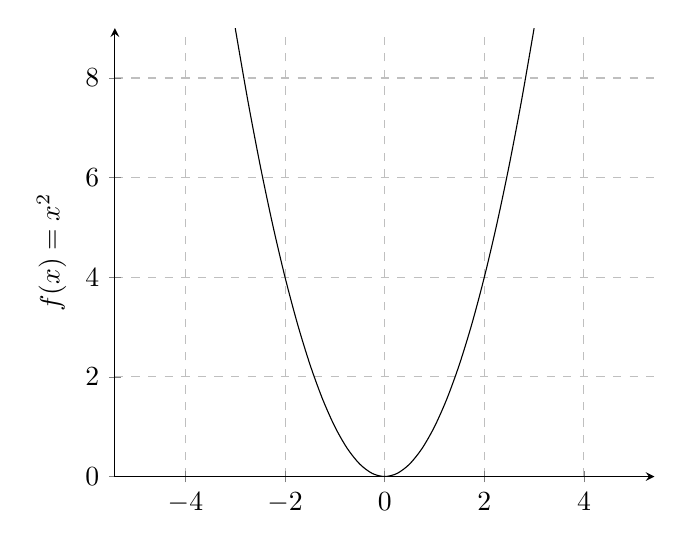
\begin{tikzpicture}
\begin{axis}[
axis x line=bottom,
axis y line = left,
%enlargelimits=true,
%xlabel=$x$,
ylabel={$f(x) = x^2$},
grid=major,
grid style=dashed,
axis equal,
]
%
use TeX as calculator:
\addplot[domain=-3:3,smooth] {x^2};
\end{axis}
\end{tikzpicture}
\end{center}

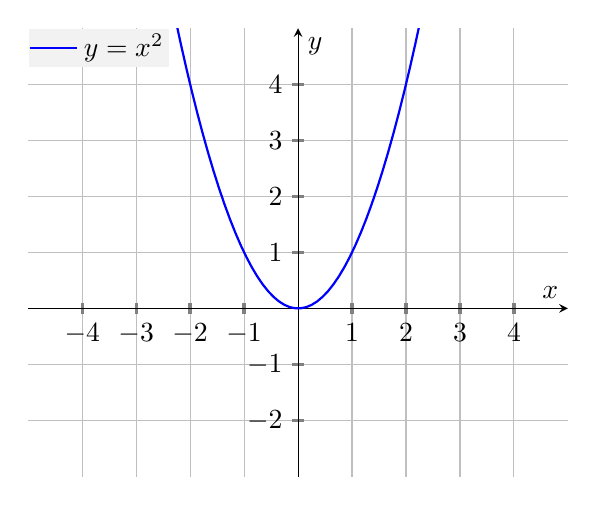
\begin{tikzpicture}
\begin{axis}[
  axis lines=middle,
  grid=major,
  xmin=-5,
  xmax=5,
  ymin=-3,
  ymax=5,
  xlabel=$x$,
  ylabel=$y$,
  xtick={-4,-3,...,4},
  ytick={-2,-1,...,4},
  tick style={very thick},
  legend style={
  at={(rel axis cs:0,1)},
  anchor=north west,draw=none,inner sep=0pt,fill=gray!10}
]
\addplot[blue,thick,samples=100] {x^2};
\addlegendentry{$y=x^2$}
\end{axis}
\end{tikzpicture}

\begin{center}
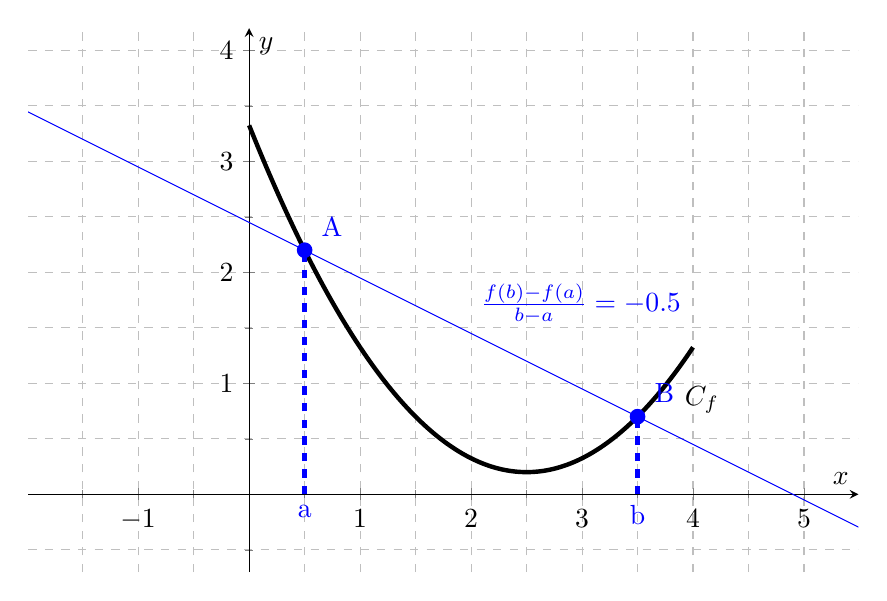
\begin{tikzpicture}[scale=1]
\begin{axis}[
axis x line=bottom,
axis y line = left,
axis lines=middle,
width=\linewidth,
height=0.7*\linewidth,
xmin=-0.5, xmax=4,
ymin=-0.5, ymax=4,
enlargelimits={abs=0.2},
xlabel={$x$},
ylabel={$y$},
minor x tick num=1,
minor y tick num=1,
%ytick distance=1,
grid=both,
grid style=dashed,
axis equal,
legend pos=north east,
]
\addplot[samples=101,smooth,ultra thick,domain=(0:4),mark=none]{0.5*(x-2.5)^2+0.2} node [pos=0.95,below right] {$\mathscr C_f$};

\node[color=blue,circle,minimum size=1pt,fill,inner sep=2pt,label={[blue]30:B}] (B) at (3.5,0.7) {};
\node[color=blue,circle,minimum size=1pt,fill,inner sep=2pt,label={[blue]30:A}] (A) at (0.5,2.2) {};
\draw [color=blue,shorten >=-5cm,shorten <=-5cm] (A)--(B) node[pos=0.5,above right] {$\frac{f(b)-f(a)} {b-a}=-0.5$};
%\addplot +[mark=none,color=blue,thick,domain=-10:10] {-0.5*x+2.45};
\addplot +[mark=none,color=blue,style=dashed,ultra thick] coordinates {(0.5,0) (0.5, 2.2)} node[pos=0,below] {a};
\addplot +[mark=none,color=blue,style=dashed,ultra thick] coordinates {(3.5,0) (3.5, 0.7)} node[pos=0,below] {b};
%\addplot +[mark=none,color=blue] coordinates {(0.5,2.2) (3.5, 0.7)} node[pos=0,circle, minimum size=1pt,fill,inner sep=2pt] {} node[pos=0,above right] {A} node[pos=1,circle, minimum size=1pt,fill,inner sep=2pt] {} node[pos=1,above] {B} node[pos=0.5,above right] {$\frac{f(b)-f(a)} {b-a}=-0.5$};
%\draw [green, ->] (2, 2) -- ++(axis direction cs:0,-1.5);
%\addlegendentry{$f(x)=x^2-x+1$};
%\pgfplotsinvokeforeach{-1.5,-1,...,2.5}{ \node[circle, minimum size=2pt,fill,color=red,inner sep=2pt] at (axis cs:#1,#1*#1-#1) {};}

%\addplot +[mark=none,color=blue,style=dashed,very thick] coordinates {(2.15, 0) (2.15, 2.47)} node [pos=0,below right] {$x$};
%\addplot +[mark=none,color=blue,style=dashed,very thick] coordinates {(2.15, 2.47) (0, 2.47)} node [pos=1,left] {$f(x)$};
%\node[circle, minimum size=1pt,fill,color=blue,inner sep=2pt] at (axis cs:2.15,2.47) {};
%\addplot +[mark=none,color=red,style=dashed,very thick] coordinates {(-1, 0) (-1, 2)};
%\addplot +[mark=none,color=red,style=dashed,very thick] coordinates {(-1, 2) (0, 2)};
%\node[label={0:{$(0,1)$}},rectangle,fill,inner sep=2pt] at (axis cs:0,1) {};
%\node[label={[label distance=2pt]-90:{$(0,1)$}},rectangle,fill,inner sep=0pt, minimum height=0pt, minimum width=4pt] at (axis cs:1,1) {};
\end{axis}
\end{tikzpicture}
\end{center}

\end{comment}


\end{document}
